% This is the root file of the thesis: thesis.tex

%%===================================
% \documentclass[12pt, oneside]{report}
\documentclass[12pt, twoside]{report}

\usepackage{url}
\usepackage[utf8]{inputenc} % This defines the font-encoding you prefer to use
\usepackage[pdftex]{graphicx}
\usepackage[bindingoffset=1cm,centering,includeheadfoot,margin=2cm]{geometry}

\usepackage[
    citestyle=numeric-comp,
    backend=biber,
    bibencoding=inputenc
    ]{biblatex}
\addbibresource{refs.bib}

\usepackage{setspace}
\linespread{1.5}
\setcounter{tocdepth}{2} 
\usepackage[colorlinks=true, pdfstartview=FitV,
linkcolor=blue, citecolor=blue, urlcolor=blue]{hyperref}
\setlength{\parindent}{0pt} % No indentation between paragraphs
\setlength{\parskip}{10pt} % Space between paragraphs

% Tables
\usepackage{ltxtable}
\usepackage{booktabs}

% Needed for code listings
\usepackage{listings}
\usepackage{color}

% Subfigure
\usepackage{subcaption}

\usepackage{floatpag} % to move floatpagenr to topright

% Fußnote
\usepackage[hang]{footmisc}
\setlength{\footnotemargin}{-0.8em}

\usepackage{csquotes}
\usepackage{afterpage} % needed for empty page after front

%%===================================
% Custom definitions
    
% Signal color
\definecolor{signalColor}{RGB}{164, 63, 114}
\newcommand\signal[1]{\textbf{\textcolor{signalColor}{#1}}}
    
% List with less space between items
\newenvironment{cList}{
\begin{itemize}
  \setlength{\itemsep}{0pt}
  \setlength{\parskip}{0pt}
  \setlength{\parsep}{0pt}
}{\end{itemize}}

% Enumeration with less space between items
\newenvironment{cEnum}{
\begin{enumerate}
  \setlength{\itemsep}{0pt}
  \setlength{\parskip}{0pt}
  \setlength{\parsep}{0pt}
}{\end{enumerate}}

% Space LoL
\let\Chapter\chapter
\def\chapter{\addtocontents{lol}{\protect\addvspace{10pt}}\Chapter}

% Rename listings and toc
\renewcommand{\contentsname}{Inhaltsverzeichnis}
\renewcommand{\lstlistlistingname}{List of Listings}

\begin{document}

%%========================================
% Frontmatter

%!TEX root = ../thesis.tex

%This is the front page
%%=========================================
\thispagestyle{empty}


\includegraphics[width=\linewidth]{fig/Logo_Header}
\mbox{}\\[1pc]
\begin{center}
    \huge{ \bfseries Methoden zur Beschreibung und Einordnung heterogener Hardware Infrastrukturen für Scientific Workflows}\\[2pc]

    \Large{Robert Balink}\\
    \large{robert.balink@campus.tu-berlin.de }\\[1pc]
    \large{16.Dezember 2021}\\[2pc]

    Bachelorarbeit\\
    Distributed and Operating Systems\\
    Technische Universität Berlin
\end{center}
\vfill

Erstprüfer:    Prof. Dr. habil. Odej Kao
\hfill\llap{Betreuer: Jonathan Bader}\\
Zweitprüfer: Prof. Dr. Dr. h.c. Sahin Albayrak

\afterpage{\null\thispagestyle{empty}\newpage}
 % This is the titlepage
\setcounter{page}{0}
\pagenumbering{Roman}
%!TEX root = ../thesis.tex

%This is the Preface
%%=========================================
\cleardoublepage
\section*{Eidestattliche Erklärung}
\addcontentsline{toc}{section}{Eidestattliche Erklärung}
Hiermit erkläre ich, dass ich die vorliegende Arbeit selbstständig und eigenhändig sowie
ohne unerlaubte fremde Hilfe und ausschließlich unter Verwendung der aufgeführten
Quellen und Hilfsmittel angefertigt habe.

Die selbständige und eigenständige Anfertigung versichert an Eides statt:

Berlin, den \the\day.\the\month.\the\year \newline
TODO: Unterschrift

%!TEX root = ../thesis.tex

%This is the Acknowledgment
%%=========================================
\cleardoublepage
\addcontentsline{toc}{section}{Anerkennung}
\section*{Anerkennung}

I would like to thank the following persons for their great support when writing my thesis at the Mobile Cloud Computing Research Group (MCC) at Technische Universität Berlin.

\begin{flushright}
INITIALS\\[1pc]
\end{flushright}

%!TEX root = ../thesis.tex

%This is the Summary
%%=========================================
\cleardoublepage
\addcontentsline{toc}{section}{Zusammenfassung}
\section*{Zusammenfassung}

Abstract Style

\newpage


\tableofcontents

\clearpage
\phantomsection
\addcontentsline{toc}{section}{\listfigurename}
\listoffigures

\clearpage
\phantomsection
\addcontentsline{toc}{section}{\listtablename}
\listoftables

\clearpage
\phantomsection
\addcontentsline{toc}{section}{\lstlistlistingname}
\lstlistoflistings

%%=========================================
% Mainmatter

\cleardoublepage
\setcounter{page}{0}
\pagenumbering{arabic}
%!TEX root = ../thesis.tex

\cleardoublepage
\chapter{Einführung}
\label{cha:introduction}

!Einführungstext eventuell!

%%=========================================
\section{Problematik}
\label{sec:motivation}

Für das Ausführen wissenschaftlicher Workflow Management Systeme, wie beispielsweise nextflow.io laufen verschiedene Arbeitspakete auf unterschiedlichen Computern. Die Arbeitspakete können allerdings zeitintensiv sein, da sie viele Ressourcen benötigen.
%schöner schreiben!
 Ohne das Wissen, welche Computereinheit leistungsstärker ist und diese dementsprechend nicht priorisieren zu können welcher Computer genutzt werden soll, k
Für den Anwender wäre es daher von Vorteil zu wissen, welcher Computer von Anfang an Leistungsfähiger ist. Durch dieses Wissen spart der Anwender sehr viel Zeit und kann effektiver die Arbeitspakete aufteilen.


%%=========================================
\section{Ziel}
\label{sec:goal}

Das Ziel dieser Abschlussarbeit ist es, die Performance relevanten und kritischen Bereiche des Computers ausfindig zu machen, die gängigen wissenschaftlichen Performance Metriken zu ermitteln und daraufhin ein eigenes Kommandozeilen Tool zu schreiben, welches die Werte aus dem Computer ausliest, analysiert und die Performance des Computers einschätzt in Relation zu einem Referenz Computer. Am Ende sollen die berechneten Werte validiert und gruppiert werden.



%%=========================================
\section{Interessante Latex Möglichkeiten}
\label{sec:structure}

This chapter gives a general introduction into the content of and the motivation for this thesis. This is done by initially outlining the motivation and problem in section \ref{sec:motivation}, defining the goal in section \ref{sec:goal}, and explaining the structure of the thesis in section \ref{sec:structure}.

\begin{figure}[ht]
    \centering
	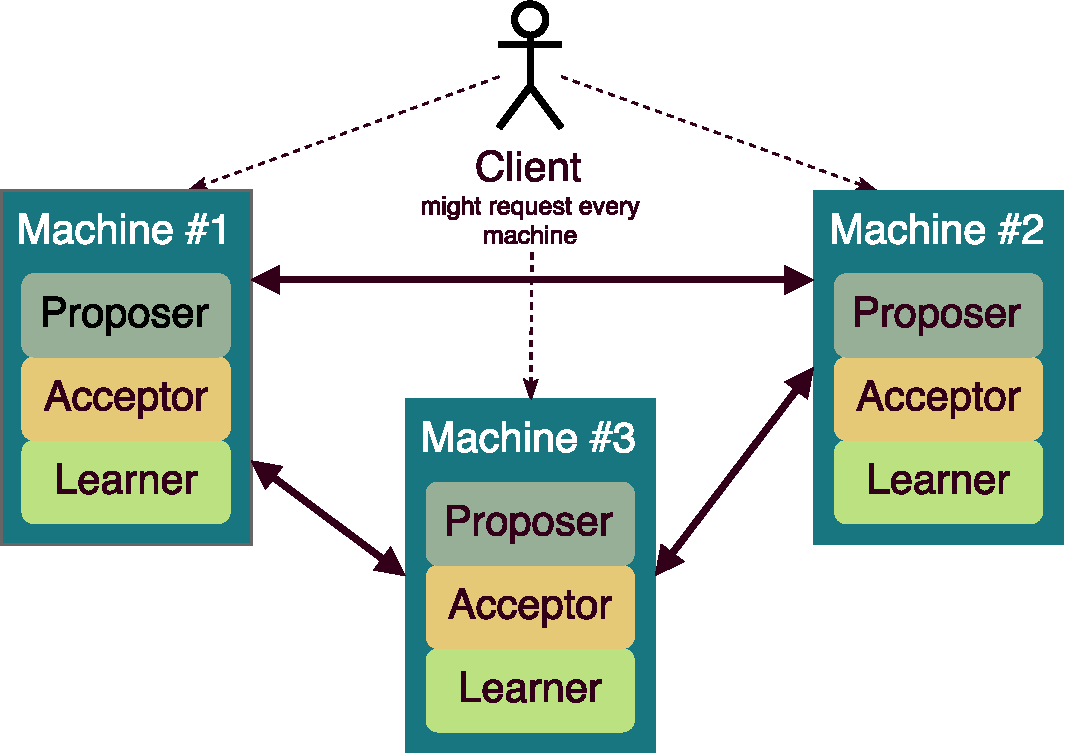
\includegraphics[width=0.8\textwidth]{fig/PaxosSetup.pdf}
	\caption{Example Setup of Three Machines Agreeing on Values Based on the Paxos Algorithm}
	\label{fig:paxosSetup}
\end{figure}

\begin{table}[ht]
    \centering
    \begin{tabularx}{\linewidth}{@{}>{\bfseries}l@{\hspace{.5em}}X@{}}
        \toprule
        \textbf{Operation related to data item} & \textbf{Consequence for vector of data item}\\ \midrule
        Update on site $S_i$ & Increment $v_i$ by one\\
        Delete or rename on site $S_i$ & Keep vector and increment $v_i$ by one, remove data item value\\
        Reconcile version conflict & Set each $v_i$ to maximum $v_i$ from all vectors used for reconciliation. In addition, increment $v_i$ of site that initiated reconciliation by one\\
        Copy to new site & Augment vector to include new site\\
        \bottomrule
    \end{tabularx}
    \caption{Influence of Operations on a Data Item's Version Vector}
    \label{tab:vectorOperations}
\end{table}

Thus, many executives feel fear to become unconscious 
Also, I want to buy \signal{smart home devices} such as the ones listed in table \ref{tab:scenario1_sensor}.

\LTXtable{\textwidth}{tab/scenario1_sensor}

\begin{cEnum}
    \item Analysis ...
    \item Design ...
    \item Prototypical implementation of the design.
\end{cEnum}

The \textbf{client}
\cleardoublepage
\chapter{Hintergrund}

%%=========================================
\section{Scientific Workflows}
\label{sec:workflows}


%%=========================================
\section{Computer Architektur}
\label{sec:architecture}

%%=========================================
\subsection{Aufbau}
\label{subsec:aufbau}

Ein moderner Personal Computer (PC) besteht aus dem Zusammenspiel von Prozessor, Arbeitsspeicher, sowie einiger Ein und Ausgabegeräten, welche untereinander mit einem Bus-System verbunden ist. Dieser Aufbau entspricht der Von-Neumann-Architektur, welche aus den 1940er Jahren stammt und vom ungarisch-amerikanischen Mathematiker John von Neumann entwickelt wurde. 
%(HAVARD ARCHITEKTUR und WARUM BESSER !
In den folgenden Unterkapiteln wird näher auf die einzelnen Bestandteile des Computers eingegangen. Allen voran dem Prozessor sowie dem Arbeitsspeicher.
Unter dem Sammelbegriff Ein und Ausgabegeräte versteht man hierbei alle Komponenten, die nicht unmittelbar zur Von-Neumann-Architektur gehören. In den folgenden Unterkapiteln wird dabei vor allem auf die Sekundärspeicher eingegangen, die eine wichtige Rolle spielen für die Performance sowie ein kurzer Überblick gegeben über die weitere typische Ein und Ausgabegeräte, die allerdings nicht von wesentlicher Bedeutung sind für die Performance.
%(Bus erklären)
ISA Bus Industry Standard Architecure
PCI Bus Peripheral Component Interconnect
%Motherboard Mainboard Hauptplatine erklären



%%=========================================
\subsection{Prozessor}
\label{subsec:cpu}

Das Herzstück des Computers bildet der Prozessor, auch CPU (Central processing unit) genannt. Der Prozessor kümmert sich um die Ausführung von Programmen, die er aus dem Arbeitsspeicher erhält. 
Die CPU besteht aus vier Funktionseinheiten. Dem Steuerwerk, dem Register, dem Rechenwerk und den Bussen.
Das Steuerwerk ist für die Koordination des gesamten Prozessors verantwortlich. Es kontrolliert hierbei die Befehle und Operationen, die das Rechenwerk als nächstes ausführen soll. 
Bei dem Register handelt es sich um Datenregister, das abhängig von ihrer Funktion unteranderem Adressen, aber auch Daten speichern kann. Sie zeichnen sich vor allem damit aus, dass auf diese Speicherbereiche schnell zugegriffen werden kann \cite{tanenbaum}. 
Das Rechenwerk, (Arithmetic Logic Unit, ALU) nutzt die vom Steuerwerk geprüften Operationen und Befehle, um diese dann auf den Daten des Registers auszuführen. Bei den Operationen und Befehlen die Verarbeitet werden handelt es sich, wie der Name ALU schon verrät um arithmetische und logische Funktionen \cite{tanenbaum}. 
Alle Komponenten sind untereinander über ein Leitungssystem, auch Bus genannt verbunden. 
De Arbeitsweise des Prozessors geht dem Abrufen-Dekodieren-Ausführen-Zyklus nach \cite{tanenbaum}.   
%(PROZESS ZEIGEN) 
--> Pipelining etwas verschnellern aber nicht wesentlich. Hierfür benötigt man mehr Prozessoren

Mehrprozessorsysteme sind Computersysteme, die mehr als einen Prozessor haben. Sie werden meist für
(MIMD /SIMD)
Statt mehr 
Horizontal und vertikal Skalieren erklären ==> Mehrprozessorsysteme vs Multicomuptersysteme
bspw Blockchain Minen
Multiprozessorsysteme --> einfach programmieren allerdings schwer zu verbinden \cite{tanenbaum} 
Multicomputersysteme --> einfacher zu bauen \cite{tanenbaum}
%hybridsystemem von beiden heute?



Durch die stetige Entwicklung von Computerchips und der damit verbundenen Erhöhung von Transistoren auf diesen steigt die Leistungsfähigkeit von Prozessoren weiter an \cite{tanenbaum}.
Fast 5 Jahrzehnte galt der Grundsatz von Gordon Moore, dass sich ungefähr alle 18 Monate die Anzahl der Transistoren pro Flächeneinheit (Integrationsdichte genannt) in einem Computerchip verdoppeln würden. Dieser Grundsatz ist als das Mooresche Gesetz bekannt. Doch auch dieses soll demnächst an seine physikalischen Grenzen kommen, da man sich im Bereich nm 
%(erklärung) 
befindet \cite{theis2017}. 

Von CPU-Herstellern wird oft die hohe Taktfrequenz beworben. Der numerische Wert lässt Endkonsumenten suggerieren, dass es sich um eine Leistungsstärkere CPU handelt. Dies ist allerdings ein Trugschluss. Eine 350 Megahertz (MHz) CPU ist nicht zwangsläufig leistungsstärker als eine CPU mit 300 MHz. Die Zahl ignoriert nämlich die tatsächliche Berechnung die bei jedem Zyklus durchgeht \cite{djl2005} 
Bei alltäglicher Nutzung eines Computers beträgt die Auslastung in den wenigsten Fällen 100 Prozent, vorallem beim Hochfahren des Computers wird die CPU unter Stress gesetzt \cite{singh2016}.
%(MEHR INFORMATIONEN)
%(Kerne )

Information über (Cache)
%(Geschwindigkeit = Clock Speed)
%RISC vs CISC


%%=========================================
\subsection{Arbeitsspeicher}
\label{subsec:memory}

Während sich der Prozessor um die Bearbeitung des Programms kümmert, befindet sich das geöffnete Programm auf dem Speicher des Arbeitsspeichers. Es bietet die Fläche für das zu bearbeitende Programm. Der Arbeitsspeicher fungiert als eine Art Zwischenspeicher, der für die Ausführung von Programme benötigt wird damit diese ausgeführt werden kann. 
%(Schöner schrieben + Brücke zwischen Festplatte und Prozessor!) 
Im Gegensatz zu einer Festplatte existieren die Daten nur zur Laufzeit und würden, wenn diese nicht im Hintergrund auf einer Festplatte hinterlegt werden alle wieder gelöscht, sobald der Computer ausgeschaltet wird. Im allgemeinen Wortgebrauch wird der Arbeitsspeicher auch als Hauptspeicher oder Memory bezeichnet. Der englische Begriff !Random Access Memory! (kurz RAM) beschreibt den Arbeitsspeicher eigentlich ziemlich treffend als !Direktzugriffsspeicher!, da dieser nämlich Zugriff auf jeden möglichen Speicherplatz des Computers hat, diesen direkt adressieren kann und im Austausch mit dem Prozessor steht \cite{haugen2000}. 
Der RAM ist wie auch der Prozessor elementarer Bestandteil 
Der Arbeitsspeicher ist aufgebaut als eine Anordnung von vielen Zellen welche Bits in sich halten, (0 oder 1) \cite{haugen2000}.  %(Erklärung RAM Aufbau und Binär)

Im Gegensatz zu Prozessoren, die sich in ihrer Leistung und damit ihrer Geschwindigkeit steigern, bekommen Arbeitsspeicher immer mehr Kapazität \cite{tanenbaum}. Technisch wäre es zwar möglich den Arbeitsspeicher auch deutlich schneller zu machen, allerdings wäre das unnötig, da die Verbindung über den Bus zwischen dem Arbeitsspeicher und dem Prozessor zu langsam ist um. Für die Optimierung der Zugriffsgeschwindigkeit nutzt man daher den sogenannten Cache (bedeutung), einen Speicher der direkt in oder neben dem Prozessor eingebaut ist \cite{tanenbaum}. Der Cache ist ein kleiner und schneller speicher der die am häufig verwendesten (Wörter?) aufbewahrt um eine schnellere Zugriffszeit für die CPU \cite{tanenbaum}. 
Während bei dem Prozessor die Geschwindigkeit untereinander verglichen werden kann, ist bei dem Arbeitsspeicher vor allem wichtig, dass die Kapazität der Programmanforderung entspricht. Sollte dies nämlich nicht der Fall sein und das Programm benötigt mehr Speicher als der Arbeitsspeicher vorweisen kann, wird die Festplatte benötigt, was dazu führt, dass der gesamte Prozess schlagartig verlangsamt wird \cite{singh2016}  %(MEHR INFO WIESO DAS DER FALL IST WENN RAM ÜBERLAUF). 
Giakamozis (1999) \cite{haugen2000} vergleicht den Arbeitsspeicher mit dem Kurzzeitgedächtnis eines Menschen, während der Sekundarspeicher das Langzeitgedächtnis repräsentiert. Sollte etwas nicht im Kurzzeitgedächtnis sein, müsste 
%(umformulieren: If short-term memory fills up, your brain sometimes is able to refresh it from facts stored in long-term memory. A computer also works this way. If RAM fills up, the processor needs to continually go to the hard disk to overlay old data in RAM with new, slowing down the computer's operation.)
Von daher ist es beim Arbeitsspeicher wichtig, genug Kapazität bereitzustellen. Ansonsten wird der RAM zum Flaschenhals des. Der leistungsstärkste Prozessor bringt einem keinen Mehrwert, wenn der Arbeitsspeicher nicht genug Platz anbietet.

%Speicherhierarchie von TANEN S.99 ! + Zugriffsgeschwindigkeit
DDR
Wenn der Arbeitsspeicher vollausgelastet ist, wird die Festplatte genutzt, was den gesamten Prozess extrem verlangsamt \cite{singh2016}.
Je langsamer der Speicher --> desto mehr Zyklen muss die CPU warten \cite{tanenbaum}




%%=========================================
\subsection{Sekundärspeicher}
\label{subsec:hdd}

Als Sekundärspeicher werden alle weiteren Speichermedien zusammengefasst, die im Gegensatz zum Arbeitsspeicher nicht in unmittelbarer Verbindung zum Prozessor stehen. Der Sekundärspeicher kann im Gegensatz zum RAM die Daten persistent speichern. 
Der Sekundärspeicher steht in Verbindung mit dem Arbeitsspeicher und kann zum Interagieren mit diesem Daten Lesen und Schreiben.
In der von-Neumann-Architektur gehören Sekundärspeicher zu den Ein und Ausgabegeräten.
Typische eingebaute Sekundärspeicher im Computer ist die Festplatte, auch Hard Drive Disk (kurz HDD) genannt, sowie die Solid State Drive (kurz SSD). Weitere Sekundärspeicher wären beispielsweise CDs, DVDs, Blu-rays, USB-Sticks oder auch Disketten. Im Gegensatz zum Arbeitsspeicher ist die Kapazität der eingebauten Sekundärspeichern enorm, dafür allerdings die Zugriffszeit deutlich langsamer. 
%(BEISPIEL ZAHLEN)
Hauptaugenmerk liegt hier vor allem bei den Festplatten und SSDs. Eine Festplatte ist ein magnetisches Speichermedium
bestehen aus mehreren runden Aluminiumscheiben mit magnetisierbarer Beschichtung \cite{tanenbaum}
% (erklärung was genau wie gespeichert wird) sie gibt es schon seit den 1950er Jahren. 
SSDs sind im Gegensatz zu Festplatten %(Flash-Speicher). 
Solid State Drive’s sind deshalb auch deutlich schneller als HDDs %(Tabelle vergleich)
Zugriffszeiten
Daher sind SSDs im Jahr 2021 auch vierfach so teuer wie HDDs für die gleiche Kapazität %(Überprüfen ob vierfach)
%(RAID = TANEN)
zugriffszeit vergrößert sich
Auch in den nächsten Jahren wird sie die Kapazität von Festplatten und SSDs vergrößern.
Wesentliche Erkenntnis für die Sekundärspeicher ist, dass für den gesamten Prozess die Zugriffsgeschwindigkeit von wichtiger Bedeutung ist, da diese ansonsten zum Flaschenhals werden kann. Neben der Zugriffsgeschwindigkeit muss selbstverständlich auch dafür gesorgt werden, dass auf dem Medium genügend Speicher vorhanden ist, um die Daten persistieren zu können.


%%=========================================
\subsection{Weitere Ein und Ausgabegeräte}
\label{subsec:inout}

Da unter dem Sammelbegriff Ein und Ausgabegeräte im Grunde alle Geräte inbegriffen sind, die in der von-Neumann-Architektur nicht in unmittelbarer Verbindung zum Prozessor stehen gibt es hier viele Beispiele für Ein und Ausgabegeräte.
Beispielhafte Eingabegeräte, die wohl die meisten Computer besitzen sind hierbei: Maus, Tastatur oder auch Mikrofon.
Ausgabegeräte wären beispielsweise Monitor, Drucker oder Lautsprecher.
Ein weiteres Ausgabegerät, welches sich typischerweise in Computern befindet und für alle Anwender wichtig ist, ist die Grafikkarte. Ohne die Grafikkarte, auch Videokarte oder Graphics processing unit (kurz GPU) genannt, würde man kein Bild auf dem Monitor angezeigt bekommen. Es ist die Schnittstelle über die Menschen mit dem Computer interagieren können. Wie bei einer CPU befindet sich in einer Grafikkarte ein Mikroprozessor. Während GPUs vor über einem Jahrzehnt hauptsächlich nur in der Lage waren 3D-Rendering-Prozesse zu verarbeiten, verfügen Grafikkarten Prozessoren mittlerweile über enorme arithmetische Kapazitäten, die sogar die CPU übertreffen \cite{owens2008}. Sie sind optimiert für das parallele Berechnen von repetitiven arithmetischen Aufgaben, wie das Darstellen von Pixeln in einem Computerspiel. Die Grafikkarte muss nämlich ununterbrochen jede Visualisierung in einem Computerspiel berechnen. In den letzten Jahren kamen vor allem zwei weitere Trends hinzu, für die sich die Funktionsweise der GPU als vorteilhaft erwiesen hat und das, obwohl diese Aufgaben keine grafischen sind. Das ist auf der einen Seite das sogenannte Minen für Blockchains, wie die Kryptowährung Bitcoin und auf der anderen Seite die Berechnung für künstliche neuronaler Netze von Machine Learning Prozessen \cite{schlegel2015} \cite{taylor2017}. Die Kombination aus Parallelisierung und der starken arithmetischen Kapazität des Mikroprozessors der Grafikkarte macht sie daher sehr beliebt für Prozesse die enorm viele Aufgaben berechnen muss.
Gewöhnliche Office-Computer oder Laptops benötigen dahingegen nicht die zusätzliche Grafikleistung und haben daher einen integrierten Grafikprozessor auf der Hauptplatine oder in der CPU direkt integriert. Dieser reicht aus, wenn keine grafisch intensiven Arbeiten verrichtet werden.


%%=========================================
\subsection{Zusammenspiel der Komponenten für die Performance}
\label{subsec:together}

technologischer Fortschritt
Auch wenn der Prozessor hauptsächlich für die Performance verantwortlich ist, so sind die anderen Komponenten im Zusammenspiel dennoch wichtig für die Gesamt-Performance des Computers.
Während sich Prozessoren durch ihre Geschwindigkeit überbieten können. Kommt es bei den Speichermedien vor allem auf die Mindestkapazität (Arbeitsspeicher) und die Zugriffszeit (Sekundärspeicher) an. Sie sind also weniger ein Beschleuniger der CPU Leistung, sondern vielmehr potentielle Flaschenhälse, welche sich negativ auf die gesamte Performance auswirken können.


%%=========================================
\section{Metriken}
\label{sec:metrics}

%%=========================================
\subsection{Anforderungen an eine Metrik}
\label{subsec:metrics}

Die Bewertungskriterien für einen Performance Test werden in einer Metrik festgehalten. Allerdings erweist es sich nicht als trivial nach welchen Kriterien die Leistung eines Computers bewertet werden soll, da kein wissenschaftlicher Konsens bis dato herrscht. Historisch betrachtet gibt es dementsprechend sowohl Unklarheiten als auch Uneinigkeiten über die richtige Methodik, da Metriken oftmals missverständlich interpretiert werden oder auch falsch angewendet wurden \cite{djl2005}. Daher stellt sich die Frage, was eine aussagekräftige Metrik für Voraussetzungen haben muss. 
Nach David J Lilja sollte eine Metrik folgendes mitbringen:
- Linear
- Zuverlässig 
- Wiederholbar
- Einfachheit der Messbarkeit
- Konsistenz
- Unabhängigkeit
nach Huppler 
- Relevanz
- Wiederholbar
- Fair and Portable
- Verifizierbar
- Economical

Eine faire und repräsentative Benchmark ist wichtig \cite{kounev2020} (2020SSB)

Schon im Jahr 1988 \cite{smith1988} (1988JES) galt es als kontrovers die Performance eines Computers auf eine einzige Zahl zu reduzieren, da man sich im wissenschaftlichen Diskurs einig war, dass die Performance multidimensional ist und sich daher durch mehrere Zahlen repräsentiert \cite{smith1988}

Wie in dem CPU-Kapitel ausgeführt, bietet sich die Taktfrequenz der CPU als ungeeignetes Kriterium einer Metrik an, da ein höherer Megahertz-Wert keine sinnvolle Aussage trifft über die Performance \cite{djl2005}. 


%%=========================================
\subsection{Historische Metriken}
\label{subsec:historic}

Eine historisch oft genutzte und bis heute immer noch beliebte Maßeinheit für die Berechnung der Computer Performance ist Millionen Instruktionen pro Sekunde (MIPS).
MIPS MFLOPS QUIPS
GigaFlops
CPU Performance Equation


%%=========================================
\subsection{Industrie Benchmarks}
\label{subsec:industry}

SPEC Benchmark System Performance Evaluation Cooperative
Aufgrund der verschiedenen Einheiten die 


%%=========================================
\subsection{openSource Benchmarks Metriken}
\label{subsec:opensource}

%%=========================================
\subsection{Fehlerquellen}
\label{subsec:fail}

Errors
Genauigkeit des Timers.

\cleardoublepage
\chapter{Methodik}

%%=========================================
\section{Anforderungen an das Programm}
\label{sec:programm}

Link zu dem github Projekt:
%GRAFIK PROGRAMM FLOW
Programmiersprache
Virtual Machine : Google Cloud Platform
Das Kommandozeilen Tool wurde in der Programmiersprache Java geschrieben 
%(vorteil Java: einmal kompiliert und dann fertig). 
Das Tool muss auf Linux Systemen funktionieren und soll dabei alle relevanten Hardware-Informationen des Computers auslesen, diese dann auf einer externen Datenbank speichern. %(MikroBenchmark Test?) 
Gleichzeitig soll anhand der Hardware-Informationen weitere relevante Benchmark Werte aus Hardware Datenbanken ausgelesen und ebenfalls gespeichert werden. Danach soll ein Ergebnis berechnet werden, wie schnell der Computer im Vergleich zu einem Referenz Computer performed. Es soll außerdem möglich sein, aus der Datenbank ein Gruppierung der vorhandenen Hardware Daten zu erstellen.
Für das Auslesen der Hardware Information wurden die Standard Kommandozeilen Befehle lscpu und xyz genutzt.
Als externe Datenbank zum speichern der relevanten Hardware Informationen wurde Postgresql gewählt. %(weil)
Die Datenbank lauft extern auf einer virtuellen Maschine, welche von der Google Cloud Platform bereit gestellt wurde. Somit ist es möglich das Programm überall ausführen können um die Daten zu speichern. Als Hilfstool zum bearbeiten der Datenbank wurde DBeaver genutzt. %(Datenbankschema Grafik)
Im Internet existieren eine Vielzahl von Online-Datenbanken für Hardware Informationen. Allerdings sind die meisten spezialisiert auf die Performance von Computerspielen und daher auch sehr Grafikkarten lastig. Hinzu kommt, dass keine einzige gefundene Online-Datenbank eine Programmierschnittstelle anbietet. Daher wurde die HtmlUnit Bibliothek für Java benutzt zum sogenannten scraping von Webseiten. Dies bedeutet, dass auslesen des gesamten Html Textes von Webseiten. Mithilfe des Document Object Model (kurz DOM) ist es möglich, direkt Elemente aus dem Html Text, wie beispielsweise Tabellen direkt anzusprechen und zu verarbeiten. %(Erklären) 

Es wurden zur Testen über 10 Computer genutzt. Zwar bietet Google Cloud Platform auch virtuelle Maschinen an, das Problem bei diesen ist allerdings, dass durch die virtualisierung keine standardmäßigen Hardware Komponenten genutzt werden, sondern für virtualisierung prozesse angepasste Komponenten die von den Hardware Herstellern extra entwickelt worden sind und dementsprechend auch in kaum einer Online-Datenbank zu finden sind. Hierfür wurden dennoch interne Mikrobenchmarking Tests gemacht.

http://cpudb.stanford.edu/processors : wissenschaftliche Datenbank für CPUs, allerdings SPEC Daten von 2006, sprich viele CPUs Benchmarks gar nicht vorhanden.


%%=========================================
\section{Online-Datenbanken}
\label{sec:database}

%%=========================================
\subsection{cpu-world}
\label{subsec:cpuworld}

%%=========================================
\subsection{userBenchmark}
\label{subsec:userbenchmark}

%%=========================================
\subsection{openBenchmarking}
\label{subsec:openbenchmarking}



%%=========================================
\section{Berechnung des Scores}
\label{sec:score}
\cleardoublepage
\chapter{Auswertung}

%%=========================================
\section{Validierung der Ergebnisse}
\label{sec:validation}

%%=========================================
\section{Abweichungen}
\label{sec:abweichung}

%%=========================================
\section{Klassifizierung der Ergebnisse}
\label{sec:klassification}
\cleardoublepage
\chapter{Stand der Forschung}

Während der Bearbeitung gab es einige Hürden.
Wie schon in dem Kapitel (METRIKEN) beschrieben, gibt es bis dato keine gängige Metrik die im wissenschaftlichen Diskurs angewendet wird. Vor allem (insert alte Metrik MFLOPS) wird noch genutzt wobei die Nachteile hier deutlich überwiegen. Oftmals werden in wissenschaftlichen Arbeiten wiederum eigene Metriken oder Benchmarks kriiert, so dass es oft gar nicht dazu kommen kann das sich Metriken etablieren.
(evntl auch in den Fazit/Diskussionstei)
Dadurch das Computerspiele, aber auch das Mining von Computern für Krytowährungen sehr populär geworden ist, gibt es unzählige Benchmark Werte für die Leistung der Komponenten von Computerspielen, vor allem spielt dort die Grafikkarte nochmal einen höheren Nutzen, also für (produktion / entwicklung).
Es gibt kaum wissenschaftliche Hardware Online Datenbanken. Leider gibt es dazu keine API Schnittstellen bei den restlichen Online Datenbanken, sodass die extraktion relevanter Daten deutlich aufwendiger war.

Eine spannende Thematik in dem Bereich Benchmarking liefert aber das Thema Performance Prediction durch Machine Learning Ansätze : beschrieben --> %CPU Hardware Classification and Performance Prediction using neural network and statistical learning 2020 (5 „Hersteller“ Performance Zonen)

\cleardoublepage
\chapter{Diskussion}
\cleardoublepage
\chapter{Fazit}

% Include more chapters as required.

%%=========================================
%Backmatter

\appendix
%!TEX root = ../thesis.tex

\cleardoublepage
\chapter{Test}

%!TEX root = ../thesis.tex

\cleardoublepage
\chapter{Abkürzungsverzeichnis}
\begin{description}
\item[AWS] Amazon Web Services
\item[IoT] Internet of Things
\end{description}

%!TEX root = ../thesis.tex

\cleardoublepage
\chapter{Lexikon}
\label{app:dic}

\paragraph*{Byzantine failure} A malfunction of a component that leads to the distribution of wrong/conflicting information to other parts of the system is called Byzantine failure . The name is based on the Byzantines Generals Problem, in which three Byzantine generals need to agree on a battle plan while one or more of them might be a traitor trying to confuse the others.

%!TEX root = ../thesis.tex

\cleardoublepage
\chapter{Listings}
\label{app:listings}

This is the appendix for code, that does not need to be provided directly inside the thesis.

\section{Configuration for Node A}

\lstinputlisting[caption={Configuration for Node A}, label={lst:nodeAConfig}]{listings/nodeAConfig.js}

% Include more appendices as required.

\cleardoublepage
\addcontentsline{toc}{chapter}{Literaturverzeichnis}
\defbibheading{notonline}{\chapter*{Literaturverzeichnis}}
\printbibliography[heading=notonline, nottype=online]
\defbibheading{online}{\chapter*{Literaturverzeichnis (Online)}}
\printbibliography[heading=online, type=online]

%%=============================================

\end{document}
